\documentclass[../main.tex]{subfiles}

\usepackage{blindtext}

\begin{document}

% AFBEELDINGEN
% pas de breedte aan door '0.25' te veranderen. 0.25 = 25% van de pagina

% foto in de tekst
% de L betekent dat hij links tevoorschijnkomt
% een R is dan natuurlijk rechts
\begin{wrapfigure}{L}{0.25\textwidth}
  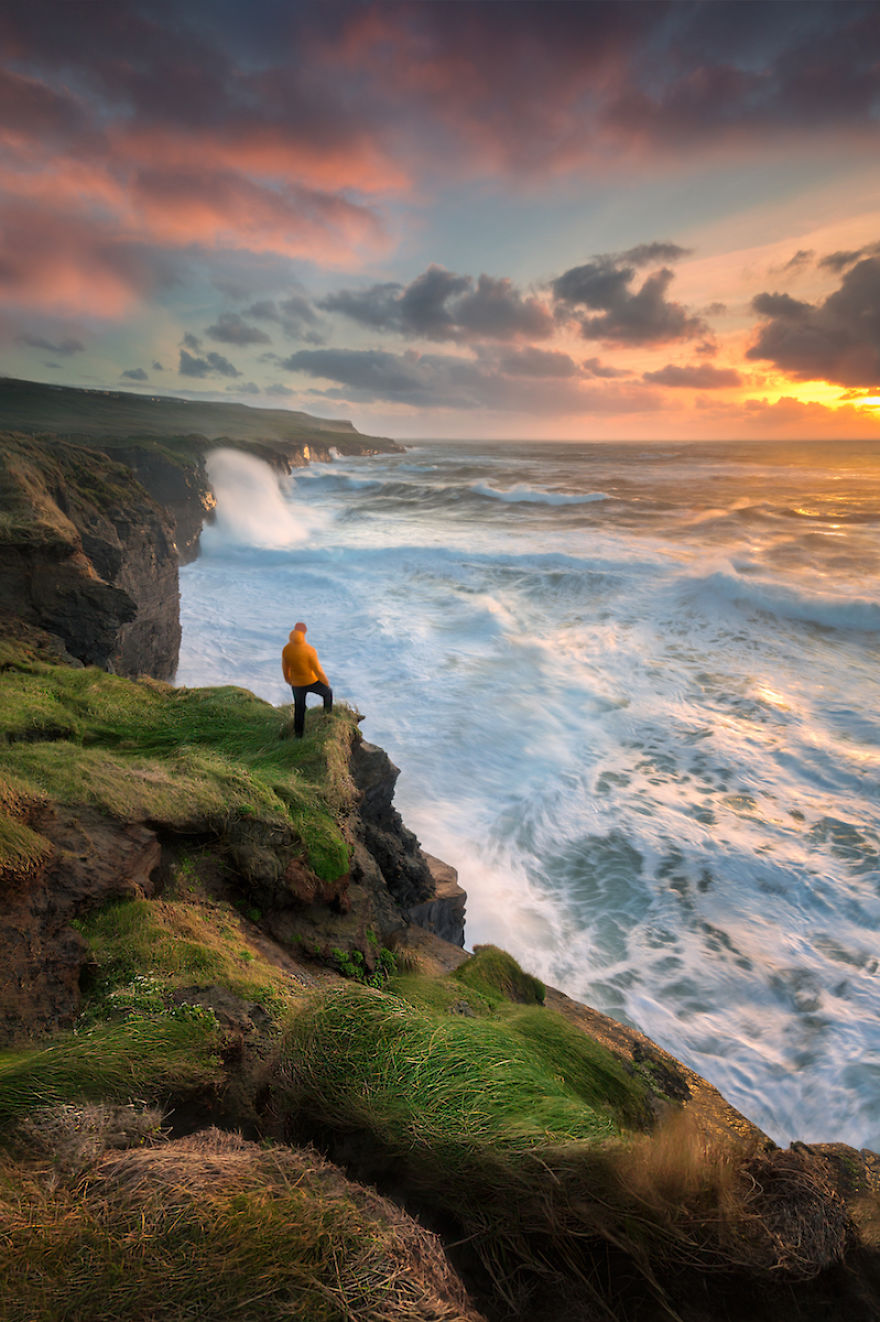
\includegraphics[width=\linewidth]{images/picture.jpg}
  \caption{Cliffs} % optioneel
\end{wrapfigure}

\blindtext

% foto onder of boven tekst
\begin{figure}[h]
  \centering
  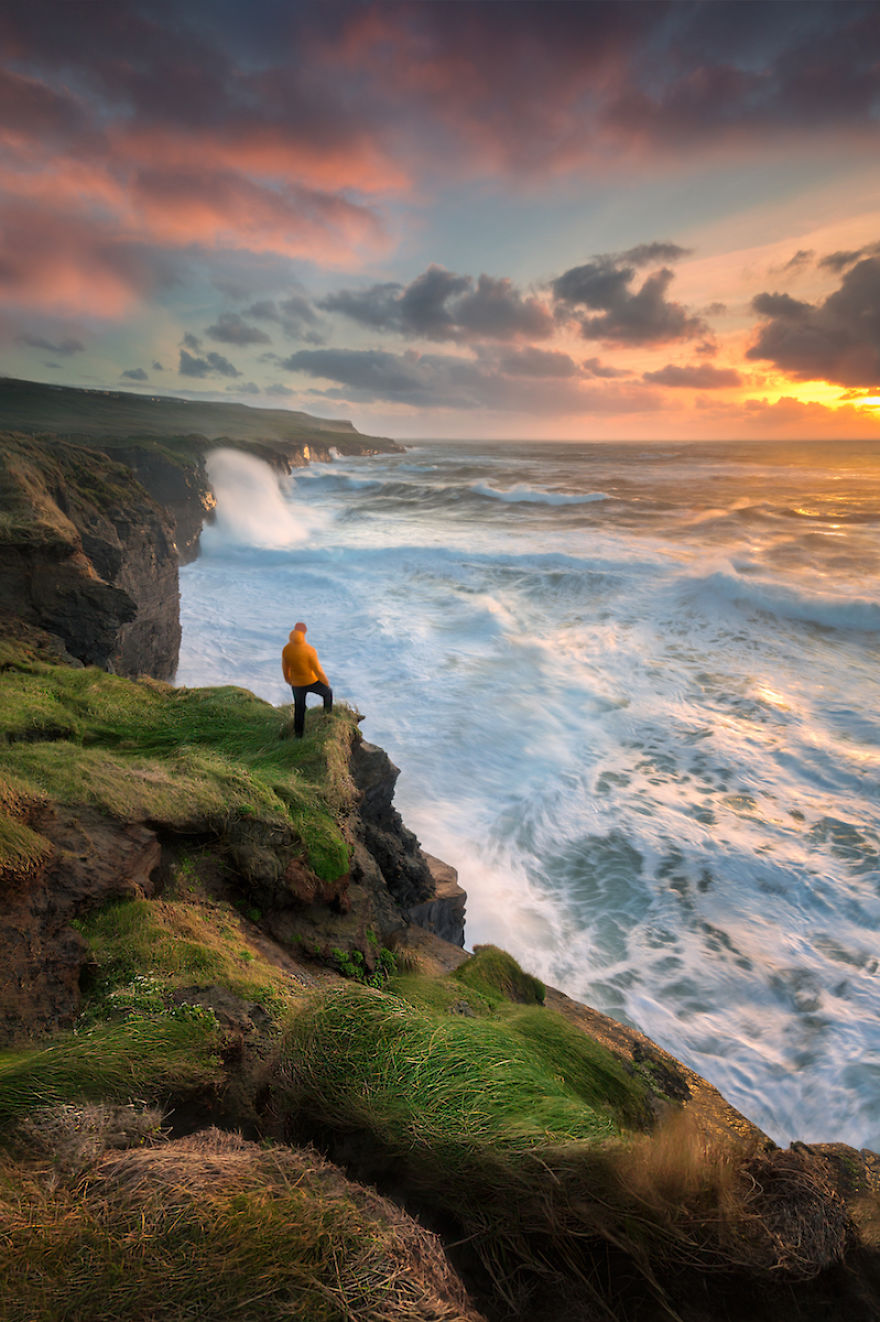
\includegraphics[width=0.25\linewidth]{images/picture.jpg}
  \caption{Cliffs} % optioneel
\end{figure}

\blindtext

\end{document}